\documentclass[12pt,a4paper,oneside,onecolumn]{book}
\usepackage[utf8]{inputenc}

%%%%%%%%%%%%%%%%%%%%%%%%%%%%%%%%%%%%%%%%%%%%%%%%
% remove unnecessary warnings
\usepackage{silence}
\WarningFilter{caption}{Unknown document class}
\WarningFilter{hyperref}{Token not allowed in a PDF string}
\WarningFilter{nameref}{The definition of \label has changed!}

%%%%%%%%%%%%%%%%%%%%%%%%%%%%%%%%%%%%%%%%%%%%%%%%
% Tell babel not to use hyphenation for Hebrew
\makeatletter\let\l@hebrew\l@nohyphenation\makeatother
% Add Hebrew:
\usepackage[hebrew,english]{babel}

%%%%%%%%%%%%%%%%%%%%%%%%%%%%%%%%%%%%%%%%%%%%%%%%
% Set page numbering with no headers (according to guidelines):
\usepackage{fancyhdr}
\pagestyle{fancy}
\lhead{}
\chead{\thepage}
\rhead{}
\lfoot{}
\cfoot{}
\rfoot{}
\renewcommand{\headrulewidth}{0pt}
\fancypagestyle{plain}{\pagestyle{fancy}}
\setlength{\headheight}{15pt}


% Misc packages:
\usepackage{textcomp} %loaded before "gensymb" to avoid annoying warnings
\usepackage{gensymb} %Degree symbol
\usepackage{mathtools} %cases*
\usepackage{amssymb} %Math letters
\usepackage[shortlabels]{enumitem}
\usepackage[multiple]{footmisc}
\usepackage{url}

\usepackage{xcolor}   %Required: \textcolor in \TODO, \fcolorbox on the open-tasks page

% Disabled to cut compile time -- nothing in the compiled chapters uses it.
% Re-enable if a code listing is added later.
%\usepackage{listings}
%\definecolor{codegreen}{rgb}{0,0.6,0}
%\definecolor{codegray}{rgb}{0.3,0.3,0.3}
%\definecolor{codepurple}{rgb}{0.5,0,0.8}
%\definecolor{backcolour}{rgb}{0.97,0.97,0.97}
%\lstdefinestyle{mystyle}{
%    backgroundcolor=\color{backcolour},   
%    commentstyle=\color{codegreen},
%    keywordstyle=\color{magenta},
%    numberstyle=\tiny\color{codegray},
%    stringstyle=\color{codepurple},
%    basicstyle=\ttfamily\scriptsize,
%    breakatwhitespace=false,         
%    breaklines=true,                 
%    captionpos=b,                    
%    keepspaces=true,                 
%    numbers=none,                    
%    numbersep=5pt,                  
%    showspaces=false,                
%    showstringspaces=false,
%    showtabs=false,                  
%    tabsize=2
%}
%\lstset{style=mystyle}

%%%%%%%%%%%%%%%%%%%%%%%%%%%%%%%%%%%%%%%%%%%%%%%%
% Misc:
\DeclareMathOperator*{\argmax}{arg\,max}
% Disabled to cut compile time -- nothing in the compiled chapters uses it.
% Re-enable if a algorithm2e is added later.
%\usepackage[ruled,vlined,algochapter]{algorithm2e}

%% algorithm2e keywords
%\SetKwInput{KwInput}{Input}

% Disabled: unused in this thesis, and costly to load.
%\usepackage{csquotes}

% Show numbers also for subsubsection
\setcounter{secnumdepth}{4}

%%%%%%%%%%%%%%%%%%%%%%%%%%%%%%%%%%%%%%%%%%%%%%%%
% bibliography:

% Author-year citations per supervisor's preference: names + dates are
% clearer for readers and referees, and work better if the material is
% later ported to a journal that permits author-year.
\usepackage[authoryear,square]{natbib}
\bibliographystyle{plainnat}

% Numeric alternative (unused; kept for reference):
% \usepackage[numbers,sort,compress,square]{natbib}
% \bibliographystyle{bibliography/unsrtnat_adjusted_for_bgu_thesis}

%add bib to toc
\usepackage[nottoc]{tocbibind}

%add command for citation with possessive apostrophe
\newcommand\citepossessive [1]{\citeauthor{#1}'s\ \cite{#1}}

%Natbib cites cannot be broken into two lines 
\makeatletter
\def\NAT@spacechar{~}% NEW
\makeatother

%%%%%%%%%%%%%%%%%%%%%%%%%%%%%%%%%%%%%%%%%%%%%%%%
% paragraph settings:
\setlength{\parindent}{0pt}
\setlength{\parskip} {5pt}

%%%%%%%%%%%%%%%%%%%%%%%%%%%%%%%%%%%%%%%%%%%%%%%%
% drawing and graphics:
% Disabled to cut compile time -- nothing in the compiled chapters uses it.
% Re-enable if a tikz is added later.
%\usepackage{tikz}
%\usepackage{tikzsymbols}
%\usetikzlibrary{matrix,positioning}
%\usetikzlibrary{shapes,positioning,calc,arrows,arrows.meta,circuits.logic.US}

\usepackage{float} %Not sure it will be needed

\usepackage{graphicx}
\graphicspath{ {content/images/} }

%%%%%%%%%%%%%%%%%%%%%%%%%%%%%%%%%%%%%%%%%%%%%%%%
% Tables
\usepackage{booktabs}   %Professional rules: \toprule, \midrule, \bottomrule
\usepackage{tabularx}   %Auto-width X columns
\usepackage{array}      %Column type modifiers (>{...})
\usepackage{multirow}   %Cells spanning several rows
\usepackage{makecell}   %Multi-line cell content via \makecell
\usepackage{longtable} %Tables that break across pages

%%%%%%%%%%%%%%%%%%%%%%%%%%%%%%%%%%%%%%%%%%%%%%%%
% DRAFT-ONLY ANNOTATIONS
% One switch controls the open-tasks page (Main_pages/todo) after the
% front matter and every inline \TODO{} marker. Set \showtodosfalse
% for a clean submission PDF.
\newif\ifshowtodos
\showtodosfalse         % <-- set to \showtodostrue while drafting

\newcommand{\TODO}[1]{\ifshowtodos\textcolor{red}{\textbf{[TODO: #1]}}\fi}

% Review markers for this session's changes live in the source as
% "% <HERE>" comment banners, not as a macro. Grep for <HERE> to find them.

%%%%%%%%%%%%%%%%%%%%%%%%%%%%%%%%%%%%%%%%%%%%%%%%
% DRAFT BUILD: skip rendering the figures.
%
% Uncomment to replace every image with an outlined box of the same size.
% Layout and page count are unchanged; image processing is skipped, which is
% the single largest saving on a figure-heavy build.
%\setkeys{Gin}{draft}

%%%%%%%%%%%%%%%%%%%%%%%%%%%%%%%%%%%%%%%%%%%%%%%%
\usepackage{titling}
\usepackage[titletoc]{appendix}

%%%%%%%%%%%%%%%%%%%%%%%%%%%%%%%%%%%%%%%%%%%%%%%%
% Hyperlinks for TOC, LOF, LOT, cross-references, and PDF outline bookmarks:
\usepackage[hidelinks,unicode,bookmarks=true,bookmarksopen=true]{hyperref}

% Hebrew babel (rlbabel.def) patches hyperref's annotation handling and uses
% the counter \c@Hy@AnnotLevel, but only the xetex and dvipdfm drivers
% allocate it -- the pdftex driver does not. Under pdflatex that produces
% "Undefined control sequence" on every \url in the bibliography. Allocating
% it here costs nothing and is harmless if a future version allocates it too.
% MiKTeX's babel-hebrew ships an rlbabel.def that patches hyperref's
% annotation handling with dvipdfm-only code: it uses the counter
% \c@Hy@AnnotLevel, which only the xetex/dvipdfm drivers allocate, and calls
% the primitive \@pdfm@mark, which does not exist under pdftex. Under
% pdflatex both surface as "Undefined control sequence" on every \url in the
% bibliography. (Overleaf avoids this by shipping the ivritex rlbabel.def
% instead.) Allocating the counter and making the dvipdfm mark a no-op costs
% nothing under pdftex, which emits its link annotations by another route.
\makeatletter
\@ifundefined{c@Hy@AnnotLevel}{\newcounter{Hy@AnnotLevel}}{}
\@ifundefined{@pdfm@mark}{\newcommand{\@pdfm@mark}[1]{}}{}
\makeatother

% For parentheses in sub-figure reference
\usepackage[labelformat=simple]{subcaption}
\renewcommand\thesubfigure{(\alph{subfigure})}

% For parentheses before sub-table caption
\renewcommand\thesubtable{(\alph{subtable})}

%%%%%%%%%%%%%%%%%%%%%%%%%%%%%%%%%%%%%%%%%%%%%%%%
%theorem, corollary, and lemma definitions:

% Disabled: unused in this thesis, and costly to load.
%\usepackage[amsmath, thmmarks, hyperref]{ntheorem}

%\newtheorem{theorem}{Theorem}
%\newtheorem{corollary}[theorem]{Corollary}
%\newtheorem{lemma}[theorem]{Lemma}
%\newtheorem{proposition}[theorem]{Proposition}
%\newtheorem{observation}[theorem]{Observation}
%\newtheorem{assumption}[theorem]{Assumption}

%%%%%%%%%%%%%%%%%%%%%%%%%%%%%%%%%%%%%%%%%%%%%%%%%
%%proof definition:

%\theoremstyle{nonumberplain}
%\theoremheaderfont{\itshape}
%\theorembodyfont{\normalfont}
%\theoremseparator{.}
%\theoremsymbol{\ensuremath{\square}}
%\newtheorem{proof}{Proof}

%% Change back to default values - needed to repeat assumptions
%\theoremstyle{plain}
%\theoremheaderfont{\normalfont\bfseries}
%\theorembodyfont{\itshape}
%\theoremseparator{}
%\theoremsymbol{}

%\usepackage{chngcntr}
%\counterwithin{theorem}{chapter}

%%%%%%%%%%%%%%%%%%%%%%%%%%%%%%%%%%%%%%%%%%%%%%%%
% cleveref:
% Disabled: unused in this thesis, and costly to load.
%\usepackage[capitalise]{cleveref}
%\crefformat{equation}{Equation #2#1#3}
%\crefformat{figure}{Figure #2#1#3}
%\crefformat{section}{Section #2#1#3}

%%Workaround for babel and cleveref (for citing few equations)
%\makeatletter
%\def\@@number#1{#1}
%\makeatother

%\Crefname{observation}{Observation}{Observations}
%\Crefname{assumption}{Assumption}{Assumptions}
%%%%%%%%%%%%%%%%%%%%%%%%%%%%%%%%%%%%%%%%%%%%%%%%
%For Hebrew table of contents: (\addcontentsline is used to add section and subsections to the Hebrew toc. For some reason, the page number is reversed only for chapter, thus we use \addtocontents for them)
\makeatletter
\newcommand\hebrewtableofcontents{%
  \selectlanguage{hebrew}%
  \section*{\contentsname
    \@mkboth{%
      \MakeUppercase\contentsname}{\MakeUppercase\contentsname}}%
 \@starttoc{tocheb}%
  \selectlanguage{english}%
 }
\makeatother

% Compatibility: in newer TeX Live releases this macro may be undefined.
\providecommand{\PrerenderUnicode}[1]{}
\PrerenderUnicode{א}

\newcommand{\onlythesecnum}{\arabic{section}}
\newcommand{\onlythesubsecnum}{\arabic{subsection}}
\newcommand{\onlythethirdsecnum}{\arabic{subsubsection}}
\newcommand{\chapnumforhebrewtoc}{\thechapter}
\newcommand{\secnumforhebrewtoc}{\onlythesecnum.\thechapter}
\newcommand{\subsecnumforhebrewtoc}{\onlythesubsecnum.\onlythesecnum.\thechapter}

%%%%%%%%%%%%%%%%%%%%%%%%%%%%%%%%%%%%%%%%%%%%%%%%
%set spacing between lines
\usepackage{setspace}
\doublespacing

%%%%%%%%%%%%%%%%%%%%%%%%%%%%%%%%%%%%%%%%%%%%%%%%
% User-editable thesis metadata is centralized here.
% Edit thesis_metadata.tex to update title, author, advisors, and date.
%%%%%%%%%%%%%%%%%%%%%%%%%%%%%%%%%%%%%%%%%%%%%%%%
% THESIS METADATA (EDIT THIS FILE)
%
% These values are reused in cover pages, abstracts, and signature pages.
% Filled from the thesis proposal (August 2025) unless marked otherwise.
%
% STILL TO CONFIRM before submission:
%   - the submission month/year (currently set to the expected date)
%   - the Hebrew title (translated here; have it checked)
%   - the Hebrew month name (currently the Gregorian month in Hebrew)
%%%%%%%%%%%%%%%%%%%%%%%%%%%%%%%%%%%%%%%%%%%%%%%%

% Thesis title
\newcommand{\thesistitle}{\large \textbf{Predicting Clinical Outcomes and
Assessing the Effects of Diabetes Care Guidelines Compliance in Hospitals
Using Temporal-Abstraction-Interval Based Transformers
and Time-Dependent Machine Learning Methods}}
\newcommand{\thesistitlehe}{\textbf{חיזוי תוצאים קליניים והערכת ההשפעה של
היענות להמלצות הטיפול בסוכרת בבתי חולים באמצעות טרנספורמרים
מבוססי מקטעי הפשטה זמנית
ושיטות למידת מכונה תלויות-זמן}}

% Faculty and institute/school -- verbatim from CIS_Thesis_Template.pdf.
\newcommand{\thesisfacultyname}{The Stein Faculty of Computer and Information Science}
\newcommand{\thesisfacultynamehe}{הפקולטה למדעי המחשב והמידע ע"ש שטיין}

% Program: the template offers Computer Science or Information Systems
% Engineering. Information Systems Engineering is selected.
\newcommand{\thesisprogram}{The program in
Information Systems Engineering
\hspace{6cm}}

\newcommand{\thesisprogramhe}{התוכנית
להנדסת מערכות מידע
\hspace{6cm}}

% Student name
\newcommand{\thesisauthorname}{\textbf{Shahar Oded}}
\newcommand{\thesisauthornamehe}{\textbf{שחר עודד}}

% Advisors list in English: separate names with \and.
\newcommand{\thesissupervisername}{Prof. Yuval Shahar}

% Advisors list in Hebrew.
\newcommand{\thesissupervisernamehe}{\textbf{פרופ' יובל שחר}}

% Submission date
\newcommand{\thesismonth}{September}
\newcommand{\thesisyear}{2026}
% The template calls for the HEBREW CALENDAR date on the Hebrew pages
% ("חודש עברי שנה עברית"), not the Gregorian one. Submission falls after
% Rosh Hashanah 5787 (12 September 2026), so the Hebrew date is Tishrei 5787.
\newcommand{\thesismonthhe}{תשרי}
\newcommand{\thesisyearhe}{תשפ"ז}


\makeatletter
\newcommand{\thesis@foradvisors}[1]{%
  \def\and{\unskip, }%
  \edef\thesis@advisorlist{\thesissupervisername}%
  \@for\thesis@advisor:=\thesis@advisorlist\do{#1}%
}

\newcommand{\thesisdisplayadvisornames}{%
  \begingroup
  \def\thesis@sep{}%
  \thesis@foradvisors{%
    \thesis@sep\thesis@advisor
    \def\thesis@sep{, }%
  }%
  \endgroup
}

% Advisor signature: if Main_pages/yuval_signature.png exists, place it
% on top of the signature line so the printed page shows the actual
% autograph. Otherwise the plain underline is drawn as before.
\newcommand{\thesisadvisorautograph}{%
  \IfFileExists{Main_pages/yuval_signature.png}{%
    \makebox[3cm][l]{\raisebox{-0.4em}{
\includegraphics[height=1.4em]{Main_pages/yuval_signature.png}}}%
  }{%
    \rule{3cm}{0.15mm}%
  }%
}

% Student signature: same treatment for Main_pages/shahar_signature.png.
\newcommand{\thesisstudentautograph}{%
  \IfFileExists{Main_pages/shahar_signature.png}{%
    \makebox[3cm][l]{\raisebox{-0.4em}{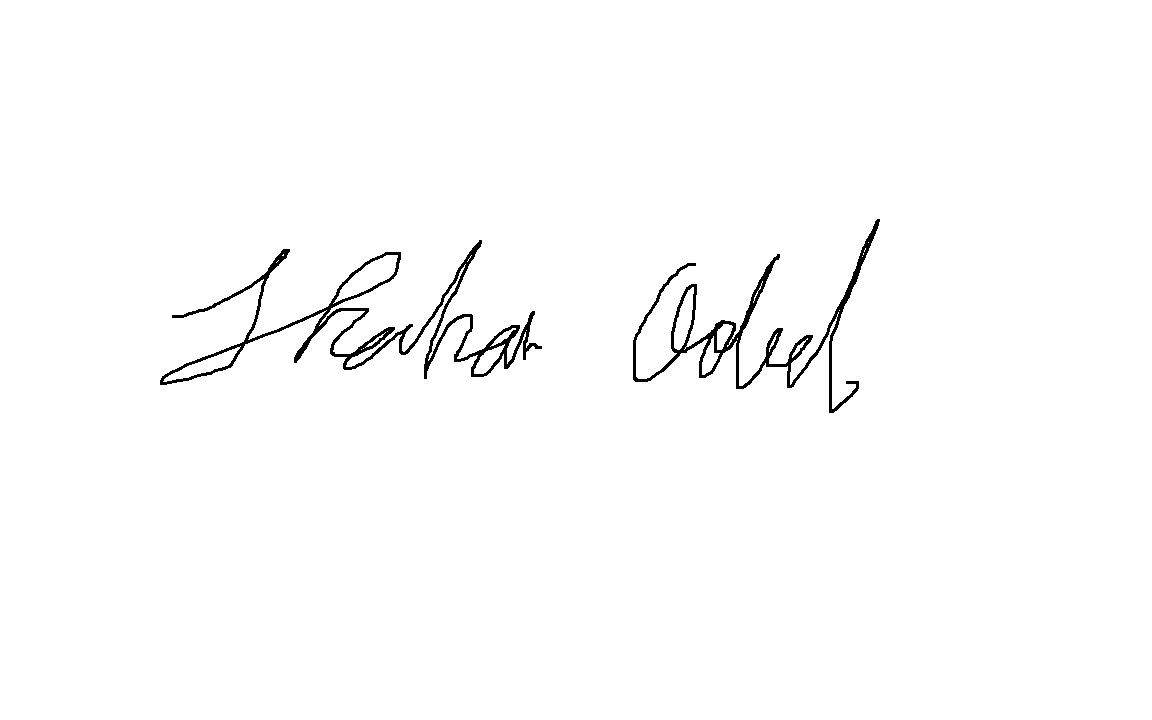
\includegraphics[height=1.4em]{Main_pages/shahar_signature.png}}}%
  }{%
    \rule{3cm}{0.15mm}%
  }%
}

\newcommand{\thesisadvisorsignatures}{%
  \begingroup
  \thesis@foradvisors{%
    Signature of advisor: \thesisadvisorautograph \hfill Date: 28/09/2026\\
  }%
  \endgroup
}

\newcommand{\thesisadvisorsignatureshe}{%
  \begingroup
  \thesis@foradvisors{%
    חתימת המנחה: \LR{\thesisadvisorautograph} \hfill תאריך: \LR{28/09/2026}\\
  }%
  \endgroup
}
\makeatother

% Reusable chapter and appendix entries.
% #1 English title
% #2 Label (without \label{})
% #3 Hebrew title for the Hebrew TOC
% #4 Input file path
%
% INCREMENTAL BUILD: add a star to skip a chapter's BODY.
%
%   \thesischapter{...}     builds the chapter in full
%   \thesischapter*{...}    emits only the heading, label and TOC entry
%
% A starred chapter still numbers correctly and its \label stays defined, so
% \ref{chapter:method} keeps working from anywhere. Only labels declared
% INSIDE a skipped chapter go undefined -- those show as '??' and are
% harmless while drafting. A red banner marks every skipped chapter in the
% PDF so a partial build can never be mistaken for a complete one.
\makeatletter

\newcommand{\thesis@stubnotice}{%
  \begin{center}
  \vspace{2em}
  \fcolorbox{red}{red!5}{%
    \parbox{0.75\textwidth}{\centering\bfseries
    \textcolor{red}{DRAFT BUILD --- this chapter's body was skipped.\\
    Remove the star from its \texttt{\char92 thesischapter*} line to include it.}}}
  \vspace{2em}
  \end{center}}

\newcommand{\thesis@head}[3]{%
  \chapter{#1}%
  \label{#2}%
  \addtocontents{tocheb}{\protect\contentsline{chapter}{\protect\numberline{\chapnumforhebrewtoc}{#3}}{{\beginL\thepage\endL}}{}}%
}

\newcommand{\thesis@full}[4]{\thesis@head{#1}{#2}{#3}\input{#4}}
\newcommand{\thesis@stub}[4]{\thesis@head{#1}{#2}{#3}\thesis@stubnotice}

\newcommand{\thesischapter}{\@ifstar\thesis@stub\thesis@full}
\newcommand{\thesisappendix}{\@ifstar\thesis@stub\thesis@full}

\makeatother
%%%%%%%%%%%%%%%%%%%%%%%%%%%%%%%%%%%%%%%%%%%%%%%%

\begin{document}

\begin{titlepage}
    % Single-spaced, with compressible gaps: the template's fixed \vspace
    % values assume a short title, and this one runs to four lines. The gaps
    % shrink only when the page would otherwise overflow, so a short title
    % still matches the template exactly.
    \singlespacing
    \begin{center}
        \vspace*{1cm plus 0pt minus 0.6cm}

        
\includegraphics[width=0.1\textwidth]{Main_pages/bgu.png}\\
        Ben-Gurion University of the Negev\\
        \thesisfacultyname\\
        \thesisprogram

        \vspace{2cm plus 0pt minus 1.2cm}

        {\Large \thesistitle}

        \vspace{1cm plus 0pt minus 0.6cm}

        Thesis submitted in partial fulfillment of the requirements\\for the Master of Sciences degree

        \vspace{1cm plus 0pt minus 0.6cm}

        \thesisauthorname

        \vspace{1cm plus 0pt minus 0.6cm}
        
        Under the supervision of\\
        \thesisdisplayadvisornames
        
        \vfill
        
        \thesismonth \quad \thesisyear

    \end{center}
\end{titlepage}
\begin{titlepage}
    % Single-spaced, with compressible gaps: the template's fixed \vspace
    % values assume a short title, and this one runs to four lines, which
    % pushed the date onto a second page. The gaps shrink only when the page
    % would otherwise overflow, so a short title still matches the template.
    \singlespacing
    \begin{center}
        \vspace*{0.7cm plus 0pt minus 0.4cm}

        
\includegraphics[width=0.1\textwidth]{Main_pages/bgu.png}\\
        Ben-Gurion University of the Negev\\
        \thesisfacultyname\\
        \thesisprogram

        \vspace{0.7cm plus 0pt minus 0.4cm}

        {\Large \thesistitle}

        \vspace{0.5cm plus 0pt minus 0.3cm}

        Thesis submitted in partial fulfillment of the requirements\\for the Master of Sciences degree

        \vspace{0.5cm plus 0pt minus 0.3cm}

        \thesisauthorname

        \vspace{0.5cm plus 0pt minus 0.3cm}

        Under the supervision of\\
        \thesisdisplayadvisornames

        \vspace{0.5cm plus 0pt minus 0.3cm}
        
        \begin{flushleft}
        Signature of student: \( \rule{3cm}{0.15mm} \) \hfill Date: 28/09/2026\\
        \thesisadvisorsignatures
        Signature of chairperson of the\\committee for graduate studies: \( \rule{3cm}{0.15mm} \) \hfill Date: \( \rule{2.5cm}{0.15mm} \)
        \end{flushleft}
        
        \vfill
        
        \thesismonth \quad \thesisyear
    \end{center}
\end{titlepage}

\frontmatter

% =====================================================================
% DRAFT-ONLY: open tasks before submission.
%
% Rendered only while \showtodostrue is set in main.tex. Carries no
% thesis content. Flipping the switch to \showtodosfalse removes this
% box and every inline \TODO{} marker at once.
% =====================================================================
\ifshowtodos
\clearpage
\thispagestyle{fancy}
\begin{center}
\fcolorbox{red}{red!4}{%
\begin{minipage}{0.92\textwidth}
\vspace{4pt}
\begin{center}
\textcolor{red}{\textbf{DRAFT --- OPEN TASKS BEFORE SUBMISSION}}
\end{center}
\vspace{2pt}
\hrule
\vspace{6pt}
\footnotesize
\singlespacing

\textbf{Acknowledgements.} \texttt{Main\_pages/acknowledgements.tex} is still
the template stub. It needs the funding source --- grant body and number, or a
statement that the work received no specific grant --- pending confirmation
from the supervisor.

\vspace{4pt}
\textbf{To flag to the supervisor.} Two points from his review were resolved
against his suggestion. The citation style stays \emph{numeric}, because the
department's template prescribes it explicitly where his structure guide asks
for author--year. And the title keeps the machine-learning framing alongside
his transformer framing, since the clinical study uses neither transformers nor
deep learning.

\vspace{4pt}
Everything else is complete. Before producing the submission PDF, set
\texttt{\char92 showtodosfalse} in \texttt{main.tex} to remove this page.

\vspace{6pt}
\end{minipage}}
\end{center}
\clearpage
\fi

\thispagestyle{plain}

% Single-spaced with tighter paragraph separation. These MUST stay inside
% \begingroup...\endgroup: \include issues a \clearpage but does not open a
% group, so without this the settings leak into the rest of the thesis and
% silently reflow every following chapter.
\begingroup
\singlespacing
\setlength{\parskip}{2pt}

\begin{center}
    \Large
    \thesistitle

    \vspace{0.2cm}
    \large
    \thesisauthorname

    \vspace{0.2cm}
    \large
    Master of Sciences Thesis

    \vspace{0.1cm}
    \large
    Ben-Gurion University of the Negev

    \vspace{0.1cm}
    \large
    \thesisyear

    \vspace{0.3cm}
    \Large
    \textbf{Abstract}
\end{center}

This thesis asks whether short-horizon complication prediction on hospitalized patients can be shaped as temporal next-token prediction over a stream of clinically named intervals, using a transformer-based model that reasons over acquired medical knowledge --- and, as a secondary goal, whether adherence to clinical guidelines governing the same care can be assessed automatically at national scale. Complications such as those governed by inpatient diabetes guidelines depend on the timely arrival of clinical data, the medical knowledge that turns those data into named concepts, and the adherence to care recommendations that connect the two. Predicting these complications, and assessing that adherence and its effect on the same complications, are the two challenges this work takes on. Both are evaluated on hospitalized patients with a diagnosis of diabetes or documented inpatient hyperglycemia. Inpatient hyperglycemia, hypoglycemia, renal failure, and other complications, including death, occur commonly in such patients and are harmful; their management is governed by clinical guidelines whose adherence is rarely measured, which is what makes automated assessment worthwhile in its own right.

A single representation addresses both objectives. A diabetes knowledge base created for the current study encodes the clinical semantics of inpatient care and the Israeli national position paper as quality-assessment temporal patterns. A temporal-abstraction engine converts an OMOP-formatted record into knowledge-based temporal abstractions and, in the same pass, scores how well the recorded care adhered to the guideline's specifications, on a scale from $0$ (lowest compliance) to $1$ (highest compliance). Every interval becomes a named clinical token, so prediction and measurement read one stream.

A \emph{methodological study} on $57{,}078$ MIMIC-IV admissions established the architecture. \textbf{INTERVenE}, a new transformer family operating natively on those intervals, comprises a bidirectional variant for single-pass prediction and an autoregressive variant that generates abstraction trajectories with per-step risk curves. Across the six target complications --- death, kidney complication, hyperglycemia, severe hyperglycemia, hypoglycemia, and severe hypoglycemia --- the encoder reached a support-weighted AUPRC of $0.672$, improving on the strongest neural baseline by $0.041$ with non-overlapping confidence intervals and on a symbolic pipeline consuming the identical interval stream by $0.085$. Sparse-transcoder attribution, computed on the deployed model through a gradient-decoupled hook, resolved every explanation to a named clinical concept. Ablations separated the sources of that gain: collapsing every interval to a point event degraded performance sharply, while replacing the clinically named intervals with an automatically derived $\sigma$-bin discretization did not. On this cohort, knowledge-based abstraction is therefore an interpretability substrate obtained at essentially no cost in accuracy rather than a predictive prerequisite.

A \emph{clinical study} on $48{,}354$ admissions across six Israeli general hospitals carried the same machinery into routine practice. Adherence levels differed by the \emph{kind} of action a recommendation required rather than by its clinical weight: recommendations satisfied by a single discrete action on admission were near-universally implemented, while those calling for repeated insulin decisions across a stay scored as low as $0.15$ and were most often entirely absent. Adherence rose modestly after implementation of a national quality measure, with marked inter-hospital heterogeneity that these data do not explain. Under propensity weighting, above-median adherence was associated with a $44\%$ lower probability of $30$-day mortality and with an $82\%$ lower probability of hyperglycemia, against a $20\%$ rise in mild hypoglycemia and no detectable rise in severe hypoglycemia --- the lopsided trade-off these recommendations are designed to strike. The recommendations that were least adhered to proved to be among those most strongly associated with outcomes.

A final experiment integrated the two studies described above. INTERVenE-Enc transferred to the clinical cohort, reaching an AUPRC of $0.527$ against $0.472$ for the strongest baseline. Here the knowledge base did carry predictive weight: the same $\sigma$-bin substitution cost $0.073$ AUPRC and left that arm level with the raw-stream baselines rather than ahead of them, so the MIMIC-IV equivalence bounds what clinical knowledge contributes when ported to a new source rather than what it contributes generally. A seven-arm ablation ran each input representation with and without the measured adherence profile supplied to the model as input. Supplying it did not shift the aggregate metrics measurably, though the interval-token arm gained $1$--$4$\,pp AUPRC on the six complications the guideline actually targets, while LogReg and set-attention baselines showed no measurable QA effect. Attribution confirmed the model reads the compliance patterns and ranks them among the top drivers for seven of eight outcomes. Adherence is largely noted implicitly through the input intervals the model had processed, and slight residual lift materializes only where attention can weight compliance patterns per outcome --- a statement about representation, not about whether following the guideline matters clinically, which the propensity-weighted analysis addressed separately, finding higher adherence consistently associated with lower mortality and reduced hyperglycemic complications after balancing measured baseline characteristics.

\endgroup

\chapter*{Acknowledgements}

This research was funded by the Israeli Ministry of Science and
Technology Kineret Grant No.~0006850 [Governmental Project
No.~1001701806], Israeli National Health Policy grant number
2020/284, the Israel Precision Medicine Partnership (IPMP) grant
No.~3543/21, and the European Union's Horizon Europe research and
innovation programme under grant agreement No.~101156210 [CARAMEL].

I am grateful to Prof.~Yuval Shahar for his supervision throughout,
and to Dr.~Erez Shalom for his technical guidance across the
software and infrastructure this work relies on. Dr.~Irit Hochberg
provided the clinical grounding for the diabetes-domain aspects of
the work; I thank her, and the clinical team she leads --- Dr.~Amir
Bashkin, Dr.~Leonard Saig, Dr.~Dror Cantrell, Dr.~Irit Wirsansky,
Dr.~Muhamad Badarne, Dr.~Irena Barash and Dr.~Avivit Cahn --- for
their input on the clinical study and for the medical guidelines carried in this research.

Finally, I thank the Kineret project team for building and maintaining
the harmonized multicenter data warehouse that made this work possible,
and for their support in accessing the data, extracting the study
cohort and exporting the results.

\vspace{1.5em}
\noindent\textbf{Ethics approval.}\quad
The clinical study reported in this thesis was approved by the institutional
Helsinki committee of each participating center under a common protocol
(NHR-0152-23): Galilee Medical Center (NHR-0152-23), Hillel Yaffe Medical
Center (HYMC-0074-24), Shamir Medical Center (ASF-0117-24), Tzafon
Medical Center (POR-0047-24), Barzilai University Medical Center
(BRZ-0059-24), and Bnai Zion Medical Center (BNZ-0067-24). A full waiver
of informed consent was granted, since the study extracts records from
a de-identified repository with no patient contact.


\tableofcontents
\clearpage

\addtocontents{tocheb}{\protect\contentsline{chapter}{\protect\numberline{}{רשימת איורים}}{{\beginL\thepage\endL}}{}}
\listoffigures
\clearpage

\addtocontents{tocheb}{\protect\contentsline{chapter}{\protect\numberline{}{רשימת טבלאות}}{{\beginL\thepage\endL}}{}}
\listoftables

%~~~~~~~~~~~~~~~~~~~~~~~~~~~~~~~~~~~~~~~~~~~~~~~~~~~~~~~~~%
\mainmatter

% User-editable chapter order (appendices are loaded further below, AFTER
% the bibliography, per supervisor's structure guidance: References print
% between chapters and appendices).
%%%%%%%%%%%%%%%%%%%%%%%%%%%%%%%%%%%%%%%%%%%%%%%%
% CHAPTERS AND APPENDICES (EDIT THIS FILE)
%
% Customize your thesis structure here.
% You can reorder, remove, or add \thesischapter lines.
%
% Chapter format:
% \thesischapter{<English title>}{<label>}{<Hebrew title for Hebrew TOC>}{<path/to/chapter_file>}
%
% Appendix format:
% \thesisappendix{<English title>}{<label>}{<Hebrew title for Hebrew TOC>}{<path/to/appendix_file>}
%%%%%%%%%%%%%%%%%%%%%%%%%%%%%%%%%%%%%%%%%%%%%%%%

%%%%%%%%%%%%%%%%%%%%%%%%%%%%%%%%%%%%%%%%%%%%%%%%
% INCREMENTAL BUILD
%
% Add a star to skip a chapter's body:  \thesischapter*{...}
% Remove it to build that chapter again.
%
% Headings, numbering and chapter labels stay correct either way, and every
% skipped chapter is marked with a red banner in the PDF.
%
% Suggested batches if the whole thesis will not compile in one pass --
% star everything except:
%   pass 1:  Introduction, Preliminaries, Related Work
%   pass 2:  Method
%   pass 3:  Evaluation, Discussion
%   pass 4:  the four appendices
%
% Remove every star for the final build.
%%%%%%%%%%%%%%%%%%%%%%%%%%%%%%%%%%%%%%%%%%%%%%%%

\thesischapter{Introduction}{chapter:intro}{מבוא}{content/introduction/introduction}
\thesischapter{Background and Related Work}{chapter:background}{רקע וסקירת ספרות}{content/background/background}
\thesischapter{Computational Methods}{chapter:comp_methods}{שיטות חישוביות}{content/method/computational_methods}
\thesischapter{Evaluation Methods}{chapter:eval_methods}{שיטות הערכה}{content/method/evaluation_methods}
\thesischapter{Results}{chapter:results}{תוצאות}{content/evaluation/evaluation}
\thesischapter{Summary, Discussion and Conclusions}{chapter:summary}{סיכום, דיון ומסקנות}{content/summary/summary}

% Example additional chapter:
% \thesischapter{Experiments}{chapter:experiments}{ניסויים}{content/experiments/experiments}

%%%%%%%%%%%%%%%%%%%%%%%%%%%%%%%%%%%%%%%%%%%%%%%%
% APPENDICES (OPTIONAL)
%
% If you do not need appendices, remove or comment out this whole block.
%%%%%%%%%%%%%%%%%%%%%%%%%%%%%%%%%%%%%%%%%%%%%%%%

\begin{appendices}

\thesisappendix{Outcome Definitions}{appendix:outcomes}{הגדרות תוצאים}{content/appendices/appendix_outcomes}
\thesisappendix{Knowledge-Base Acquisition and Validation}{appendix:kb}{רכישת בסיס הידע ותיקופו}{content/appendices/appendix_kb}
\thesisappendix{Architectural Ablation Trail}{appendix:ablations}{ניסויי אבלציה ארכיטקטוניים}{content/appendices/appendix_ablations}
\thesisappendix{Calibration, Trajectories, and Implementation}{appendix:calibration}{כיול, מסלולים ופרטי מימוש}{content/appendices/appendix_calibration}
\thesisappendix{Kineret Benchmark Detail}{appendix:kineret}{פרטי מדד ההשוואה על קינרת}{content/appendices/appendix_kineret}
\thesisappendix{Future Work}{appendix:future_work}{כיווני מחקר עתידיים}{content/appendices/appendix_future_work}

% Example additional appendix:
% \thesisappendix{Extended Proofs}{appendix:proofs}{הוכחות מורחבות}{content/appendices/extended_proofs}

\end{appendices}


%~~~~~~~~~~~~~~~~~~~~~~~~~~~~~~~~~~~~~~~~~~~~~~~~~~~~~~~~~%
\addtocontents{tocheb}{\protect\contentsline{chapter}{{ביבליוגרפיה}}{{\beginL\thepage\endL}}{}}
\bibliography{bibliography/thesis}

% Appendices after the bibliography.
%%%%%%%%%%%%%%%%%%%%%%%%%%%%%%%%%%%%%%%%%%%%%%%%
% APPENDICES (OPTIONAL)
%
% This file is loaded by main.tex AFTER the bibliography, so References
% print between chapters and appendices (supervisor's structure guidance).
%
% If you do not need appendices, remove or comment out the \input line
% in main.tex.
%%%%%%%%%%%%%%%%%%%%%%%%%%%%%%%%%%%%%%%%%%%%%%%%

\begin{appendices}

\thesisappendix{Outcome Definitions}{appendix:outcomes}{הגדרות תוצאים}{content/appendices/appendix_outcomes}
\thesisappendix{Knowledge-Base Acquisition and Validation}{appendix:kb}{רכישת בסיס הידע ותיקופו}{content/appendices/appendix_kb}
\thesisappendix{Architectural Ablation Trail}{appendix:ablations}{ניסויי אבלציה ארכיטקטוניים}{content/appendices/appendix_ablations}
\thesisappendix{Calibration, Trajectories, and Implementation}{appendix:calibration}{כיול, מסלולים ופרטי מימוש}{content/appendices/appendix_calibration}
\thesisappendix{Kineret Benchmark Detail}{appendix:kineret}{פרטי מדד ההשוואה על קינרת}{content/appendices/appendix_kineret}
% Future Work is a section of Chapter~6 (Summary, Discussion and Conclusions),
% not an appendix, per supervisor's structure guidance.

\end{appendices}


\clearpage
% no page numbering from now on
\pagenumbering{gobble} 
\hebrewtableofcontents

\thispagestyle{empty}

\selectlanguage{hebrew}

% Single-spaced, as in the English abstract.
\begingroup
\singlespacing
\setlength{\parskip}{2pt}

% Latin runs inside Hebrew are wrapped in babel-hebrew's \LR, which embeds
% them left-to-right. Without it the engine reverses them: OMOP prints as POMO.

\begin{center}
    \Large
    \thesistitlehe

    \vspace{0.25cm}
    \large
    \thesisauthornamehe

    \vspace{0.25cm}
    \large
    עבודת גמר לתואר מוסמך למדעים

    \vspace{0.1cm}
    \large
    אוניברסיטת בן-גוריון בנגב

    \vspace{0.1cm}
    \large
    \thesisyearhe

    \vspace{0.4cm}
    \Large
    \textbf{תקציר}
\end{center}

היפרגליקמיה בקרב מאושפזים היא תופעה שכיחה ומזיקה, והטיפול בה מוסדר בהנחיות קליניות שמידת היישום שלהן נמדדת לעתים רחוקות בלבד. עבודה זו בוחנת האם ניתן להעריך את מידת ההיענות להנחיות באופן אוטומטי ובקנה מידה לאומי, והאם ניתן לנסח את בעיית חיזוי הסיבוכים לטווח הקצר --- המוצגת בדרך כלל כבעיית סיווג מבוססת מאפיינים על גבי מדידות גולמיות --- כבעיית חיזוי המילה הבאה ברצף זמני, באמצעות מודל מבוסס טרנספורמר הפועל על גבי ידע רפואי נרכש.

ייצוג אחד מחבר בין שתי המטרות. בסיס ידע לטיפול בסוכרת, שנבנה במסגרת עבודה זו, מקודד את הסמנטיקה הקלינית של הטיפול באשפוז ואת נייר העמדה הלאומי הישראלי כתבניות זמניות להערכת איכות. מנוע הפשטה זמנית ממיר רשומה בתקן \LR{OMOP} להפשטות זמניות מבוססות ידע, ובאותו מעבר מחשב עד כמה הטיפול המתועד סטה ממפרט ההנחיה. כל מקטע הפשטה הופך למונח קליני מפורש, ולכן החיזוי וההערכה קוראים רצף אחד.

\emph{המחקר המתודולוגי}, על $57{,}078$ אשפוזים ממאגר \LR{MIMIC-IV}, מבסס את הארכיטקטורה. \LR{\textbf{INTERVenE}}, משפחת מודלים מסוג טרנספורמר הפועלת ישירות על מקטעי ההפשטה, כוללת וריאנט דו-כיווני לחיזוי במעבר יחיד ווריאנט אוטורגרסיבי המחולל מסלולי הפשטה עם עקומות סיכון לכל צעד. המקודד משיג \LR{AUPRC} משוקלל של $0.672$, שיפור של $0.041$ על פני קו הבסיס הנוירוני החזק ביותר עם רווחי סמך שאינם חופפים, ושל $0.085$ על פני צינור סימבולי הצורך את אותו רצף מקטעים בדיוק. שיטת ייחוס מבוססת מקודדים דלילים, המחושבת על המודל הפרוס דרך וו מנותק-גרדיאנט, מתרגמת כל הסבר למונח קליני מפורש. ניסויי אבלציה מפרידים בין מקורות השיפור: כיווץ כל מקטע לאירוע נקודתי פוגע בביצועים פגיעה חדה, ואילו החלפת המקטעים בעלי השמות הקליניים בדיסקרטיזציה אוטומטית מבוססת סטיות תקן אינה פוגעת בהם. מכאן שבקוהורט זה ההפשטה מבוססת הידע היא תשתית לפרשנות, המושגת בעלות כמעט אפסית בביצועים, ולא תנאי הכרחי לחיזוי.

\emph{המחקר הקליני}, על $48{,}354$ אשפוזים בשישה בתי חולים כלליים בישראל, מיישם את אותה מערכת בפרקטיקה השגרתית. רמות ההיענות נבדלות לפי \emph{סוג} הפעולה הנדרשת ולא לפי משקלה הקליני: המלצות המסתפקות בפעולה בדידה אחת בקבלה מיושמות כמעט תמיד, ואילו המלצות הדורשות החלטות אינסולין חוזרות לאורך האשפוז מקבלות ציונים נמוכים עד $0.15$ ולרוב נעדרות כליל. ההיענות עלתה במידה מתונה לאחר הטמעתו של מדד איכות לאומי, עם שונות ניכרת בין בתי החולים שהנתונים אינם מסבירים. לאחר שקלול הסתברות הטיפול, היענות מעל החציון נקשרה בסיכוי נמוך ב-$44\%$ לתמותה תוך $30$ יום, וגם בסיכוי נמוך ב-$82\%$ להיפרגליקמיה, לעומת עלייה של $20\%$ בהיפוגליקמיה קלה וללא עלייה מובהקת בהיפוגליקמיה חמורה --- בדיוק חילופי התועלת הלא-סימטריים שהמלצות אלו נועדו להשיג. ההמלצות שההיענות להן הייתה הנמוכה ביותר נמצאו מבין הקשורות ביותר לתוצאים.

ניסוי מסכם מחבר בין שני החלקים. \LR{INTERVenE} עוברת בהצלחה לקוהורט הקליני ומשיגה $0.527$ לעומת $0.472$ של קו הבסיס החזק ביותר. כאן בסיס הידע אכן תורם ליכולת החיזוי: אותה החלפה בדיסקרטיזציה אוטומטית עולה $0.073$ \LR{AUPRC} ומורידה את הזרוע לרמת קווי הבסיס שעל הנתונים הגולמיים, ולכן ממצא \LR{MIMIC-IV} תוחם את תרומת הידע הקליני במעבר למקור חדש ולא באופן גורף. סולם בן שבע זרועות מריץ כל ייצוג קלט עם פרופיל ההיענות הנמדד כקלט למודל ובלעדיו. הוספתו לא שינתה אף מדד באופן מובהק, אף שניתוח הייחוס מראה כי המודל אכן קורא אותו ומדרג את תבניות ההיענות מבין הגורמים המשפיעים ביותר עבור שבעה מתוך שמונה תוצאים. ההיענות מסכמת את המקטעים שהמודל כבר רואה ואינה מוסיפה עליהם --- אמירה על הייצוג, ולא על השאלה אם יש ערך קליני בהיענות להנחיה, שעליה עונה בנפרד ובחיוב הניתוח משוקלל ההסתברות.

\endgroup
\selectlanguage{english}

% The gaps below are rubber lengths: the template's fixed values assume a
% one-line title, and this thesis runs to four lines in Hebrew. They compress
% only when the page would otherwise overflow, so a shorter title renders
% exactly as the template intends.
\begin{titlepage}
    \begin{center}
        \vspace*{1cm plus 0pt minus 0.8cm}

        
\includegraphics[width=0.1\textwidth]{Main_pages/bgu.png}\\
        \selectlanguage{hebrew}
        אוניברסיטת בן-גוריון בנגב\\
        \thesisfacultynamehe\\
        \thesisprogramhe

        \vspace{1cm plus 0pt minus 0.8cm}

        {\Large \thesistitlehe}

        \vspace{0.5cm plus 0pt minus 0.35cm}

        חיבור זה מהווה חלק מהדרישות לקבלת התואר מוסמך למדעים

        \vspace{0.5cm plus 0pt minus 0.35cm}

        \thesisauthornamehe

        \vspace{0.5cm plus 0pt minus 0.35cm}

        בהנחיית\\
        \thesissupervisernamehe

        \vspace{0.5cm plus 0pt minus 0.35cm}

        \begin{flushleft}
        חתימת הסטודנט/ית: \( \rule{3cm}{0.15mm} \) \hfill תאריך: \( \rule{2.5cm}{0.15mm} \)\\
        \thesisadvisorsignatureshe
        \makebox[\linewidth][l]{חתימת יו"ר ועדת הוראה מוסמכים: \( \rule{2.6cm}{0.15mm} \) \hfill תאריך: \( \rule{2.2cm}{0.15mm} \)}
        \end{flushleft}

        \vfill

        \thesismonthhe \quad \thesisyearhe
    \end{center}
\end{titlepage}


\begin{titlepage}
    \centering
    % Title pages are single-spaced, and the vertical gaps below are rubber
    % lengths: the template's fixed values assume a one-line title, and this
    % thesis runs to three lines in Hebrew. The gaps compress only when the
    % page would otherwise overflow, so short titles look exactly as the
    % template intends.
    \singlespacing
    \vspace*{1cm plus 0pt minus 0.6cm}

    
\includegraphics[width=0.1\textwidth]{Main_pages/bgu.png}\par
    \selectlanguage{hebrew}
    אוניברסיטת בן-גוריון בנגב\par
    	\thesisfacultynamehe\par
    	\thesisprogramhe\par

    \vspace{2cm plus 0pt minus 1.20cm}

    {\Large \thesistitlehe\par}

    \vspace{1.5cm plus 0pt minus 0.90cm}

    חיבור זה מהווה חלק מהדרישות לקבלת התואר מוסמך למדעים\par

    \vspace{1cm plus 0pt minus 0.60cm}

    	\thesisauthornamehe\par

    \vspace{1cm plus 0pt minus 0.60cm}

    בהנחיית\par
    	\thesissupervisernamehe\par

    \vfill

    	\thesismonthhe\quad \thesisyearhe\par
\end{titlepage}

\end{document}